\documentclass[t]{beamer} \usefonttheme[onlymath]{serif}
\mode<presentation>
{
  \usetheme{Frankfurt}
  \usecolortheme{dove}  %% grey scale
  \useinnertheme{circles}
  \setbeamercovered{invisible}
}

\hypersetup{
    colorlinks,
    citecolor=black,
    filecolor=black,
    linkcolor=black,
    urlcolor=blue
}
\usepackage{graphicx}

\graphicspath{ {./imgs} }

% \usepackage{listings} % embed code
% \usepackage{minted} % embed code
\usepackage{color}

\setbeamertemplate{itemize}{$\circ$}
\setbeamertemplate{itemize items}{$\circ$}

\beamertemplatenavigationsymbolsempty %% no navigation bar

\setbeamertemplate{footline}{\hspace*{.1cm}\scriptsize{
\hspace*{50pt} \hfill\insertframenumber/\inserttotalframenumber\hspace*{.1cm}\vspace*{.1cm}}}

\setbeamertemplate{caption}[numbered]
\setbeamerfont{caption}{size=\tiny}


%%% Rust language
% The following configuration comes from: https://github.com/denki/listings-rust/blob/master/listings-rust.sty
%
%%%


\title{Sonobe, a modular folding schemes library}
\date{
  
\includegraphics[width=3cm]{sonobe}\\
  \vspace{0.1cm}
  \scriptsize{2024-10-08\\0xPARC \& PSE}
}

\begin{document}

\frame{\titlepage}

%%%%%
% Sketch:
%
% Anatomy of Folding Schemes
%   - Arithmetization - IVC - Decider
% Overview of Sonobe
%   diagram, frontend - folding/IVC - Decider - OnChain/OffChain verifier
% example of code switching schemes \& curves (arkworks style)
%%%%%

\section{Motivation}

\begin{frame}{Polynomials and SNARKs}
  \begin{itemize}
    \item define the 'program' that we want to be able to prove as a set of constraints
    \item encode the constraints as polynomials
    \\eg. R1CS: $Az \circ Bz - Cz == 0$
    \\~~~~~~~~~~$A(X) \cdot B(X) - C(X) == 0$
    \item and then use some scheme to prove that those polynomials satisfy the relation. eg. Groth16, Spartan, etc
  \end{itemize}
  \vspace{0.5cm}
  TL;DR: want to prove polynomial relations
\end{frame}

\begin{frame}{Why folding}
  \begin{itemize}
    \item Repetitive computations take big circuits $\longrightarrow$ large proving time
    \begin{itemize}
      \item in some cases takes too much memory and can not be even computed
      \item eg. prove a chain of 10k sha256 hashes (>600M R1CS constraints, not feasible with most traditional SNARK proving systems)
      \item eg. zkVM opcodes
    \end{itemize}

    \pause
    \item Traditional recursion: verify (in-circuit) a proof of the correct execution of the same circuit for the previous input
    \begin{itemize}
      \item issue: in-circuit proof verification is expensive (constraints)
      \begin{itemize}
        \item ie. verify a Groth16 proof inside a R1CS circuit
      \end{itemize}
    \end{itemize}
  \end{itemize}

  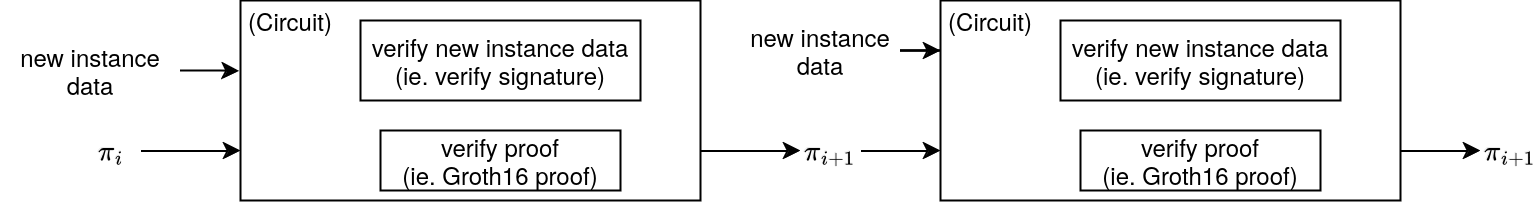
\includegraphics[width=\textwidth]{brute-force-recursion}

\end{frame}

\begin{frame}{IVC - Incremental Verifiable Computation}
  {\tiny Valiant'08}
  % Folding schemes efficitently achieve IVC, where the prover recursively proves the correct execution of the incremental computations.
  %\vspace{0.5cm}

  \emph{Prove that applying $n$ times the $F$ function (the circuit being folded) to the initial state ($z_0$) results in the final state ($z_n$).}

  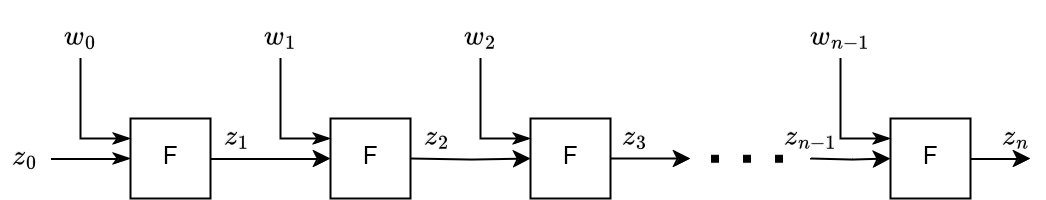
\includegraphics[width=\textwidth]{folding-main-idea-diagram}

  In other words, it allows to prove efficiently that
  $$z_n = F(...~F(F(F(F(z_0, w_0), w_1), w_2), ...), w_{n-1})$$
\end{frame}


\begin{frame}{Folding scheme pipeline}
  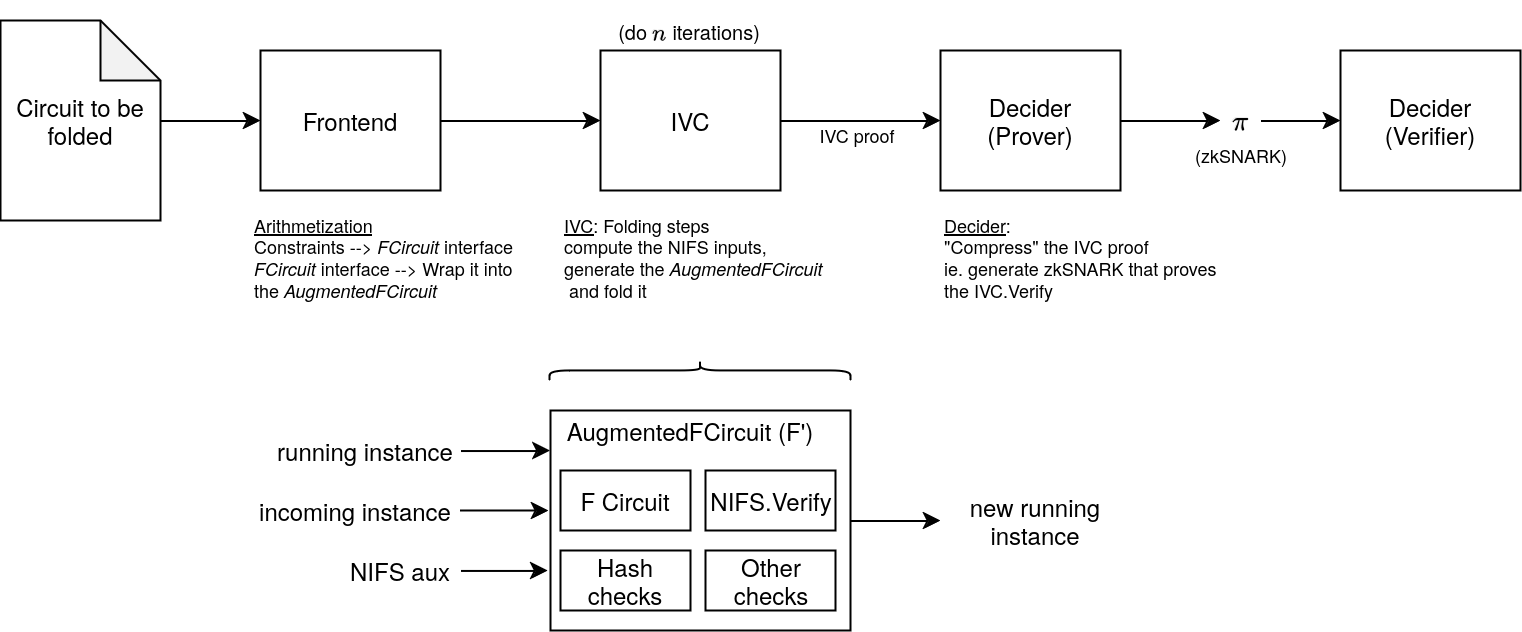
\includegraphics[width=\textwidth]{folding-scheme-pipeline}

  \vspace{0.5cm}
  {\scriptsize
  The IVC folds the AugmentedFCircuit, which ensures that the NIFS.Verify checks out.
  }
\end{frame}


\section{Recap on folding}

% TODO MAYBE REMOVE SLIDE
\begin{frame}{RLC of homomorphic commitments}
  \small{
    In the initial folding schemes, we rely on homomorphic commitments, eg. Pedersen commitments\\
  }

  Let $g \in \mathbb{G}^n,~ v \in \mathbb{F}_r^n$,\\
  $$Com(v) = \langle g, v \rangle =g_1 \cdot v_1 + g_2 \cdot v_2 + \ldots + g_n \cdot v_n \in \mathbb{G}$$

  RLC:\\
  Let $v, w \in \mathbb{F}_r^n$,
  \\set $cm_v = Com(v),~ cm_w=Com(w) \in \mathbb{G}$.
  \\then,
  \begin{align*}
    y &= v + r \cdot w\\
    cm_{y} &=cm_v + r \cdot cm_w
  \end{align*}
  \\so that
  $$cm_y = Com(y)$$
\end{frame}

% TODO MAYBE REMOVE SLIDE
%%%%%%%%%%%%%%%%% TODO maybe get rid of the slide if not enough time
%%%%
\begin{frame}{Random linearly combining 2 R1CS instances}
  \scriptsize{

    R1CS instance: $(\{A, B, C\} \in \mathbb{F}^{n \times n},~ n,~ l)$, such that for $z=(1, io \in \mathbb{F}^l, w \in \mathbb{F}^{n-l-1}) \in \mathbb{F}^n$,

    $$Az \circ Bz = Cz$$


      If we try to do a RLC with two instances ($z = z_1 + r \dot z_2$):
      \begin{align*}
        Az \circ Bz &= A(z_1 + r z_2) \circ B(z_1 + r z_2)\\
        &= (Az_1 \circ Bz_1) + r \cdot (A z_1 \circ B z_2 + A z_2 \circ B z_1) + r^2 \cdot (A z_2 \circ B z_2)\\
        &\neq C z = C(z_1 + r z_2) = C z_1 + r C z_2 = (A z_1 \circ B z_1) + r \cdot (A z_2 \circ B z_2)
      \end{align*}
      we end up with some inequality.


    \pause

    Nova's solution, Relaxed R1CS:

    $$Az \circ Bz = uCz + E$$

    for $u \in \mathbb{F},~~ E \in \mathbb{F}^n$.

    \vspace{0.5cm}

    Witness of the instance: $WI=(E, W)$\\
    Committed Relaxed R1CS instance: $CI = (\overline{E}, u, \overline{W}, x)$
  }

  \vspace{0.3cm}
  \tiny{Full details at Nova's paper, pages 13-15 ("first attempt, second attempt, third attempt")}

\end{frame}

% TODO MAYBE REMOVE SLIDE
% \begin{frame}{Relaxed R1CS}
%   % \vspace{-1cm}
%   \scriptsize{
%         $u=u_1+r u_2,~~ z=z_1+r z_2,~~ x=x_1+r x_2$\\
%         $E=E_1 + r (A z_1 \circ B z_2 + A z_2 \circ B z_1 - u_1 C z_2 - u_2 C z_1) + r^2 E_2$\\
%   \text{Relaxed R1CS:} $Az \circ Bz = uCz + E,~~ with~ z=(u,~x,~W)$
%   \begin{align*}
%           Az \circ Bz 
%               &= A(z_1 + r \cdot z_2) \circ B(z_1 + r \cdot z_2)\\
%               &= A z_1 \circ B z_1 + r(A z_1 \circ B z_2 + A z_2 \circ B z_1) + r^2 (A z_2 \circ B z_2)\\
%               &= (u_1 C z_1 + E_1) + r (A z_1 \circ B z_2 + A z_2 \circ B z_1) + r^2 (u_2 C z_2 + E_2)\\
%               &= u_1 C z_1 + \underbrace{E_1 + r(A z_1 \circ B z_2 + A z_2 \circ B z_1) + r^2 E_2}_\text{E} + r^2 u_2 C z_2\\
%               &= u_1 C z_1 + r^2 u_2 C z_2 + E\\
%               &= (u_1 + r u_2) \cdot C \cdot (z_1 + r z_2) + E\\
%               &= uCz + E
%   \end{align*}
% 
%   For R1CS matrices $(A,~B,~C)$, the folded witness $W$ is a satisfying witness for the folded instance $(E,~u,~x)$, following the Relaxed R1CS relation: $Az \circ Bz - uCz - E ==0$.
% 
%   Since we don't want that the Verifier learning about the witness, we commit to it, and the Verifier will run the RLC on the commitment (not on the witness), obtaining the 'folded' commitment.
% 
%   \\\tiny{Full details at Nova's paper, pages 13-15 ("first attempt, second attempt, third attempt")}
%   }
% \end{frame}
%%%%
%%%%%%%%%%%%%%%%%

\begin{frame}{NIFS: Non Interactive Folding Scheme (in Nova)}
  {\tiny
  Main idea:
  \begin{itemize}
    \item protocol between P (Prover) and V (Verifier)
    \item where P and V obtain the 'folded' committed instance that corresponds to the 'folded' witness instance that P computes
    \item so V does not know the witness
  \end{itemize}
  % We make it non-interactive with Fiat-Shamir.
  RelaxedR1CS relation: $Az \circ Bz = uCz + E$, for $u \in \mathbb{F},~~ E \in \mathbb{F}^n$.
  \\Witness of the instance: $WI=(E, W)$\\
  Committed Relaxed R1CS instance: $CI = (\overline{E}, u, \overline{W}, x)$

  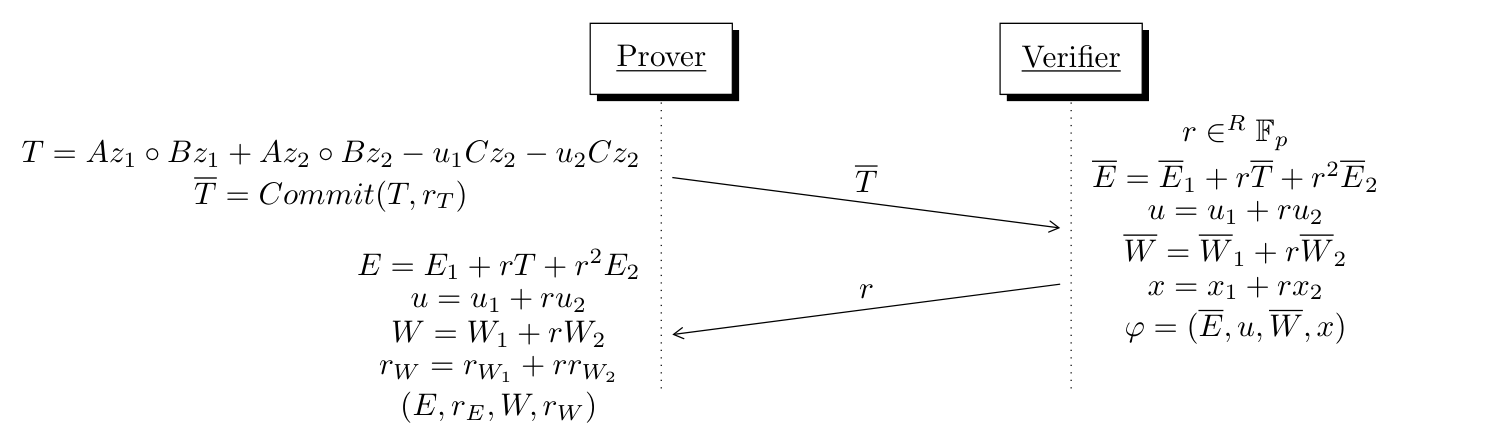
\includegraphics[width=\textwidth]{interactive-FS-nova-diagram}

  Relation check:
  \begin{align*}
    &z=(1,x,W)\\
     &\begin{cases}
    Az \circ Bz - uCz - E \stackrel{?}{=} 0\\
    \overline{W} \stackrel{?}{=} Com(W)\\
    \overline{E} \stackrel{?}{=} Com(E)
  \end{cases}
  \end{align*}
  }
\end{frame}

\begin{frame}{NIMFS}
  issue: the RLC with $>2$ instances makes the cross-terms grow
  \\ie. some vectors ($T$) would get bigger and their commitments ($\overline{T}$) more expensive

  \pause
  \vspace{0.5cm}

  NIMFS in HyperNova, ProtoGalaxy, etc
  \begin{itemize}
    \item instead of 2 RLC between 2 instances
    \begin{itemize}
      \item HyperNova: run SumCheck
      \item ProtoGalaxy: protocol using Lagrange Basis (instead of random values) for the linear combinations and then the zero-check protocol
        \\alternatively using MLE and SumCheck
    \end{itemize}
  \end{itemize}
  Allowing to fold $>2$ instances at each folding step.
\end{frame}

\begin{frame}
  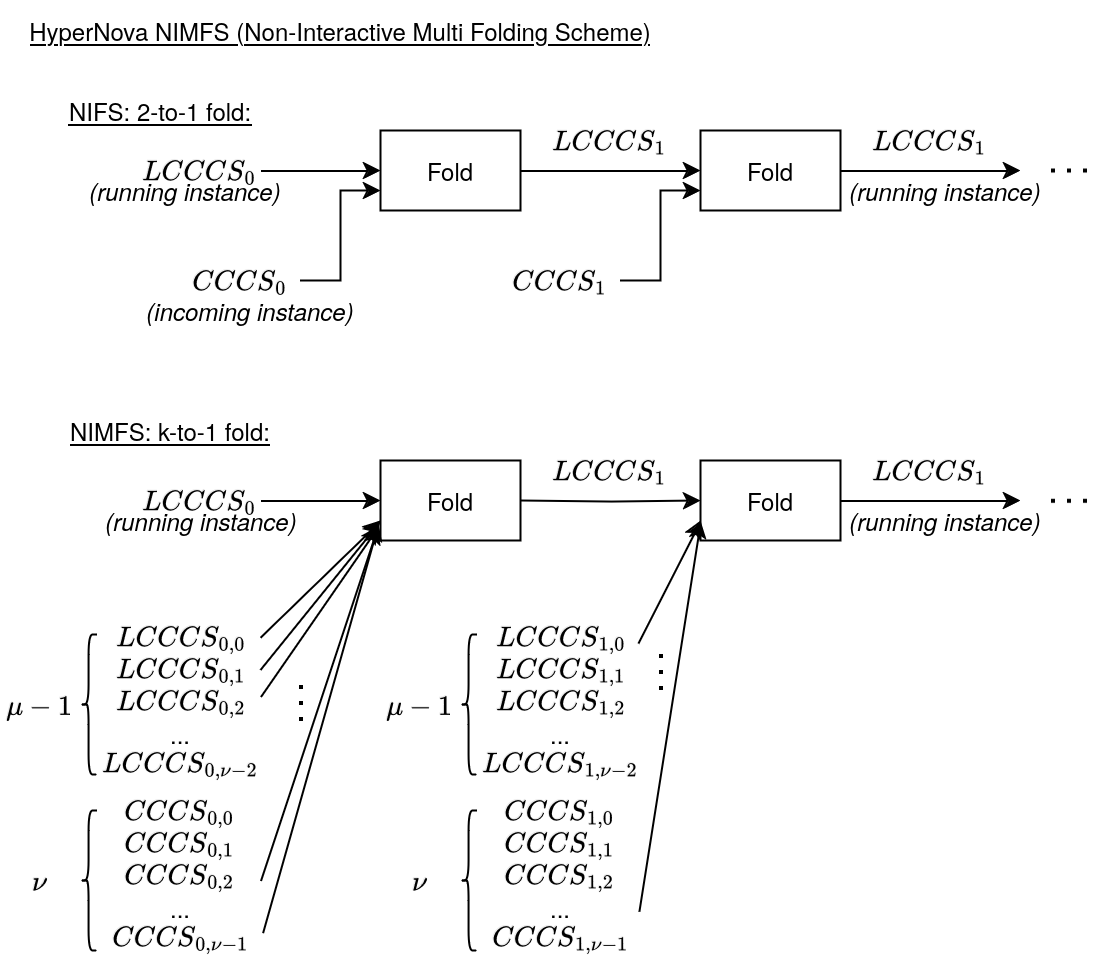
\includegraphics[height=\textheight]{multifolding-idea}
\end{frame}

\begin{frame}{HyperNova NIMFS}
  {\tiny src: \href{https://eprint.iacr.org/2023/573.pdf}{https://eprint.iacr.org/2023/573.pdf} (HyperNova paper)}
  \vspace{-0.5cm}
  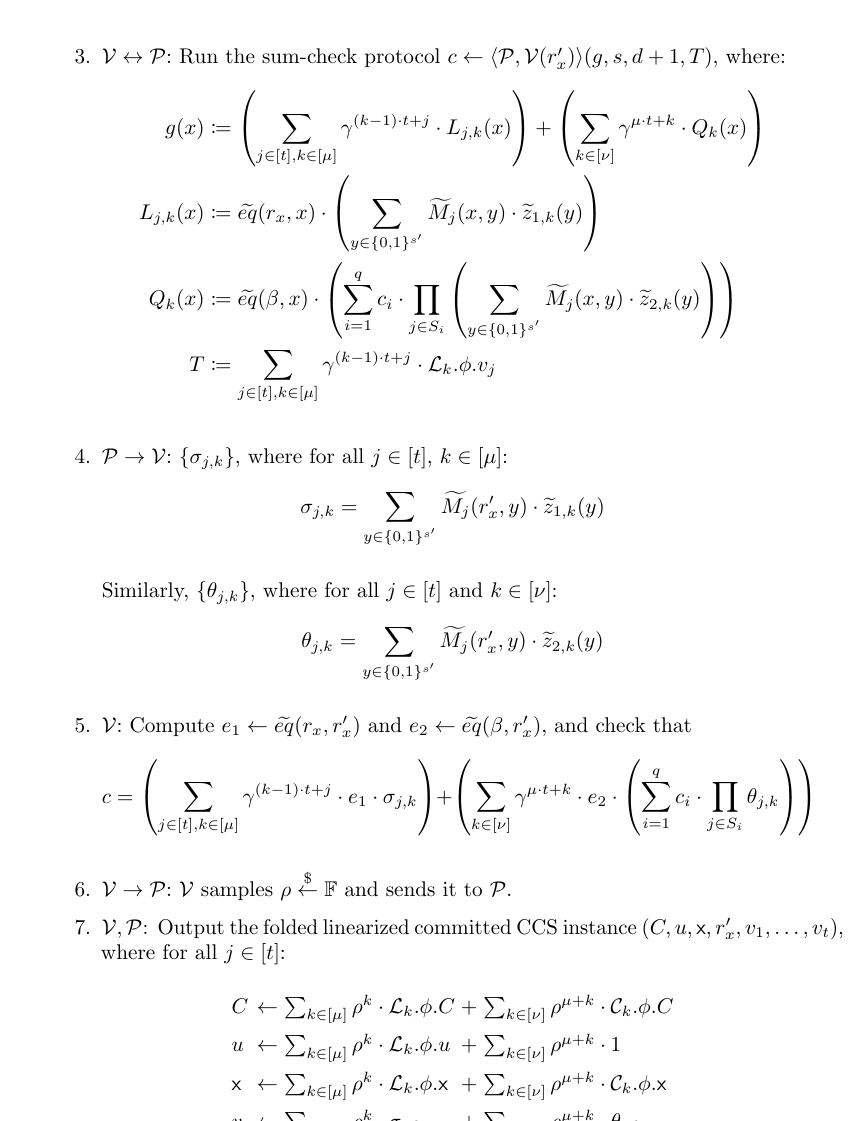
\includegraphics[width=8cm]{./imgs/hypernova-screenshot}
\end{frame}

\begin{frame}{ProtoGalaxy Folding}
  {\tiny src: \href{https://eprint.iacr.org/2023/1106.pdf}{https://eprint.iacr.org/2023/1106.pdf} (ProtoGalaxy paper)}
  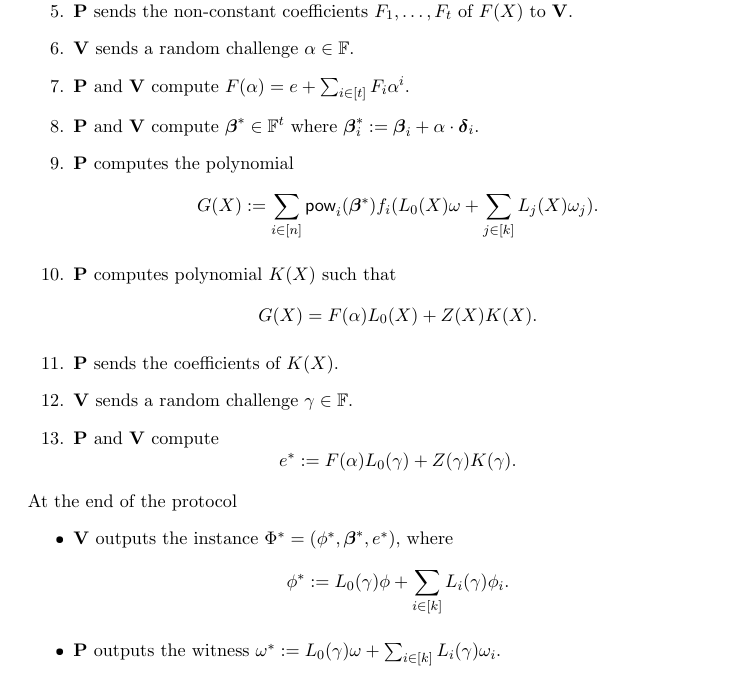
\includegraphics[width=8cm]{./imgs/protogalaxy-screenshot}
\end{frame}

\section{IVC}

\begin{frame}{(Recall) Folding scheme pipeline}
  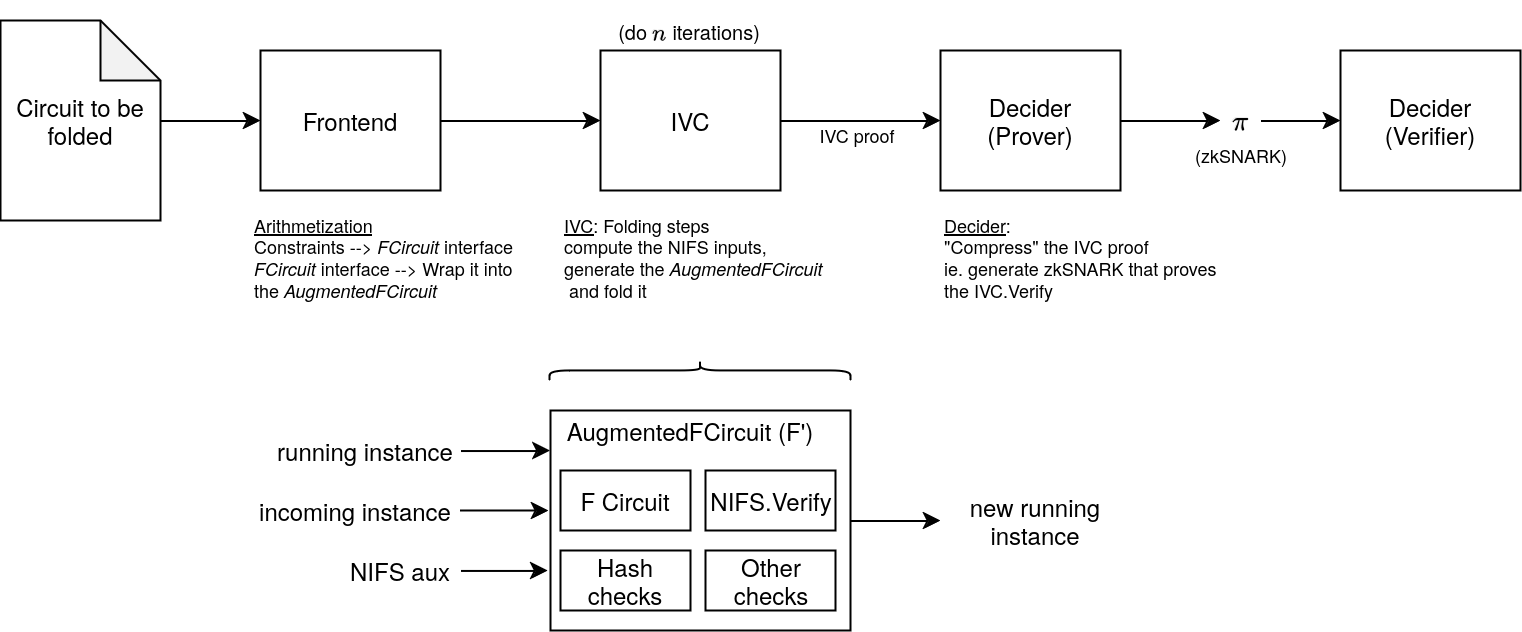
\includegraphics[width=\textwidth]{folding-scheme-pipeline}

  \vspace{0.5cm}
  {\scriptsize
  The IVC folds the AugmentedFCircuit, which ensures that the NIFS.Verify checks out.
  }
\end{frame}

% ANNOTATION:
% Now, we have this protocol between Prover and Verifier to 'fold', 'combine' 2 instances into a new instance, which if satisfies the relation checks, it means that the 2 original ones were satisfying it too.
% We're going to see now how do we convert this into

\begin{frame}{IVC - Incrementally Verifiable Computation}
  \begin{itemize}
    \item need to ensure that at each fold (IVC step), the NIFS is correctly done
    \item want to have a construction where we fold the circuit that itself contains the checks of the Folding Scheme (NIFS.Verify)
    \item we encode the NIFS.Verify inside a circuit (\emph{AugmentedFCircuit}), together with other checks that ensure the correct relations
    \item and is this \emph{AugmentedFCircuit} ($F'$) the one which we actually fold
  \end{itemize}

  % TODO rm:
  % 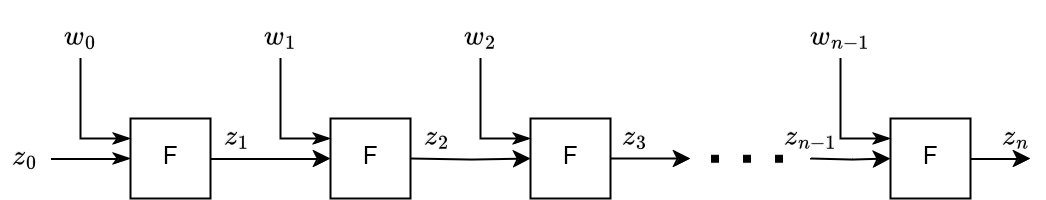
\includegraphics[width=\textwidth]{folding-main-idea-diagram}
  % $$z_n = F(...~F(F(F(F(z_0, w_0), w_1), w_2), ...), w_{n-1})$$
\end{frame}

\begin{frame}{Folding circuit - AugmentedFCircuit}
    wrapper over the circuit that we want to fold
    \begin{itemize}
      \item contains the circuit that we want to fold
      \item plus extra checks ensuring that the fold is being done correctly\\
      \begin{itemize}
        \item some hashing and values checks
        \item run the NIFS.Verify in-circuit
        \begin{itemize}
          \item Nova: RLC of $\mathbb{F}$ and $\mathbb{G}$ elements
          \item HyperNova: RLC of $\mathbb{F}$ and $\mathbb{G}$ elements + SumCheck verifier
          \item ProtoGalaxy: linear cominations of $\mathbb{F}$ and $\mathbb{G}$ elements with the Lagrange basis and some polynomial evaluations + ... (alternatively SumCheck)
        \end{itemize}
      \end{itemize}
    \end{itemize}
  

\end{frame}

\begin{frame}{Cycle of curves}
  \scriptsize{
    NIFS.V involves $\mathbb{G}$ point operation, which are not native over $\mathbb{F}_r$ of $\mathbb{G}$.
  \\$\longrightarrow$ delegate them into a circuit over a 2nd curve 
  We use:
  \begin{itemize}
    \item $\mathbb{G}_1.\mathbb{F}_r = \mathbb{G}_2.\mathbb{F}_q$
    \item $\mathbb{G}_1.\mathbb{F}_q = \mathbb{G}_2.\mathbb{F}_r$
    \item eg. for Ethereum compatibility:\\
      $\mathbb{G}_1$: BN254, $\mathbb{G}_2$: Grumpkin.
  \end{itemize}

  We 'mirror' the main $F'$ circuit into the 2nd curve\\
  each circuit computes natively the point operations of the other curve's circuit
  }
  \vspace{0.3cm}

  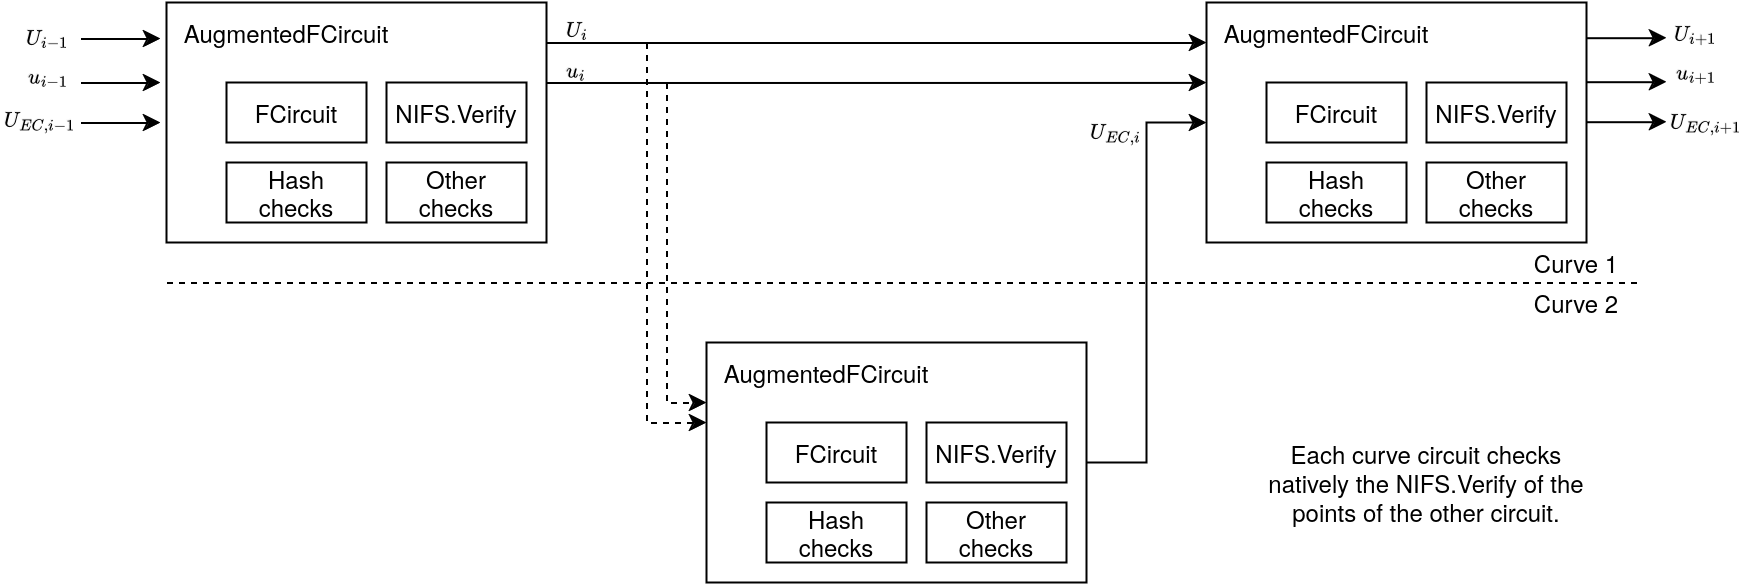
\includegraphics[width=\textwidth]{nova-cycle-of-curves-mirror}
\end{frame}

\begin{frame}{Cycle of curves}
  \scriptsize{
    NIFS.V involves $\mathbb{G}$ point operation, which are not native over $\mathbb{F}_r$ of $\mathbb{G}$.
  \\$\longrightarrow$ delegate them into a circuit over a 2nd curve 
  We use:
  \begin{itemize}
    \item $\mathbb{G}_1.\mathbb{F}_r = \mathbb{G}_2.\mathbb{F}_q$
    \item $\mathbb{G}_1.\mathbb{F}_q = \mathbb{G}_2.\mathbb{F}_r$
    \item eg. for Ethereum compatibility:\\
      $\mathbb{G}_1$: BN254, $\mathbb{G}_2$: Grumpkin.
  \end{itemize}

  We 'mirror' the main $F'$ circuit into the 2nd curve\\
  each circuit computes natively the point operations of the other curve's circuit
  }
  \vspace{0.3cm}

  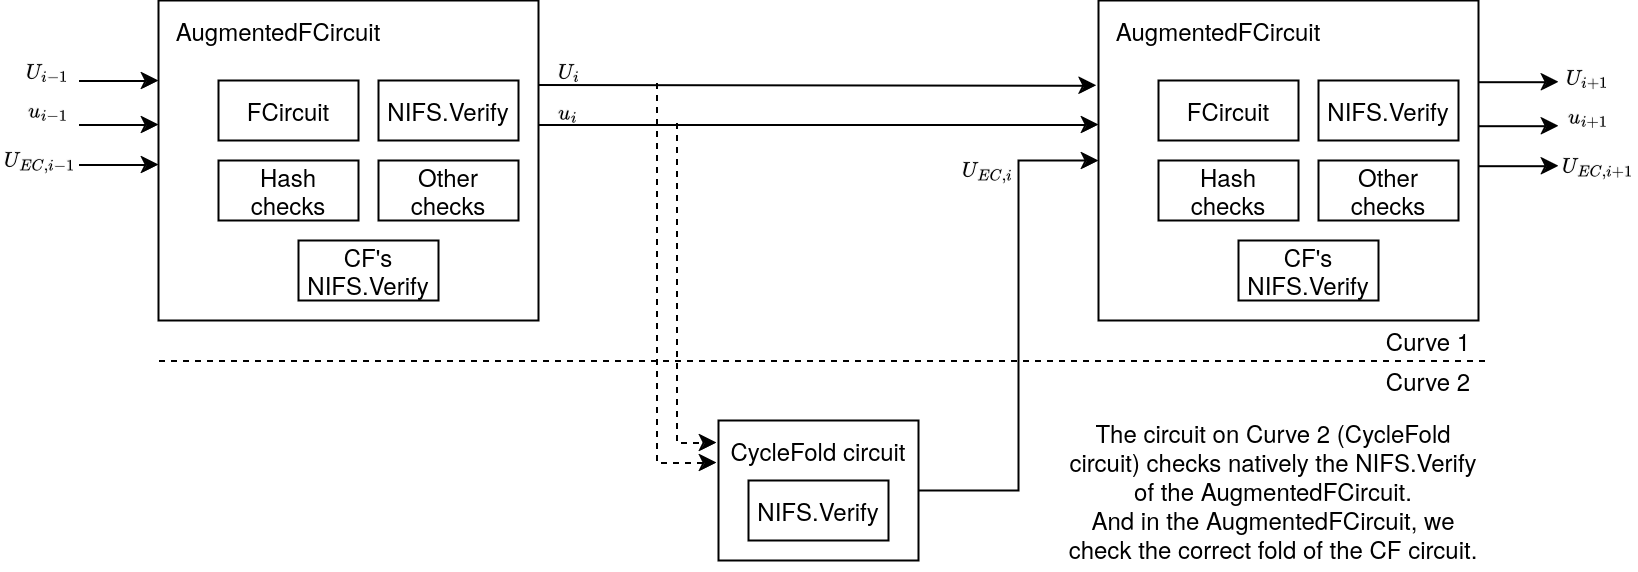
\includegraphics[width=\textwidth]{nova-cycle-of-curves-cyclefold}
\end{frame}

% slide with only the image:
{
\usebackgroundtemplate{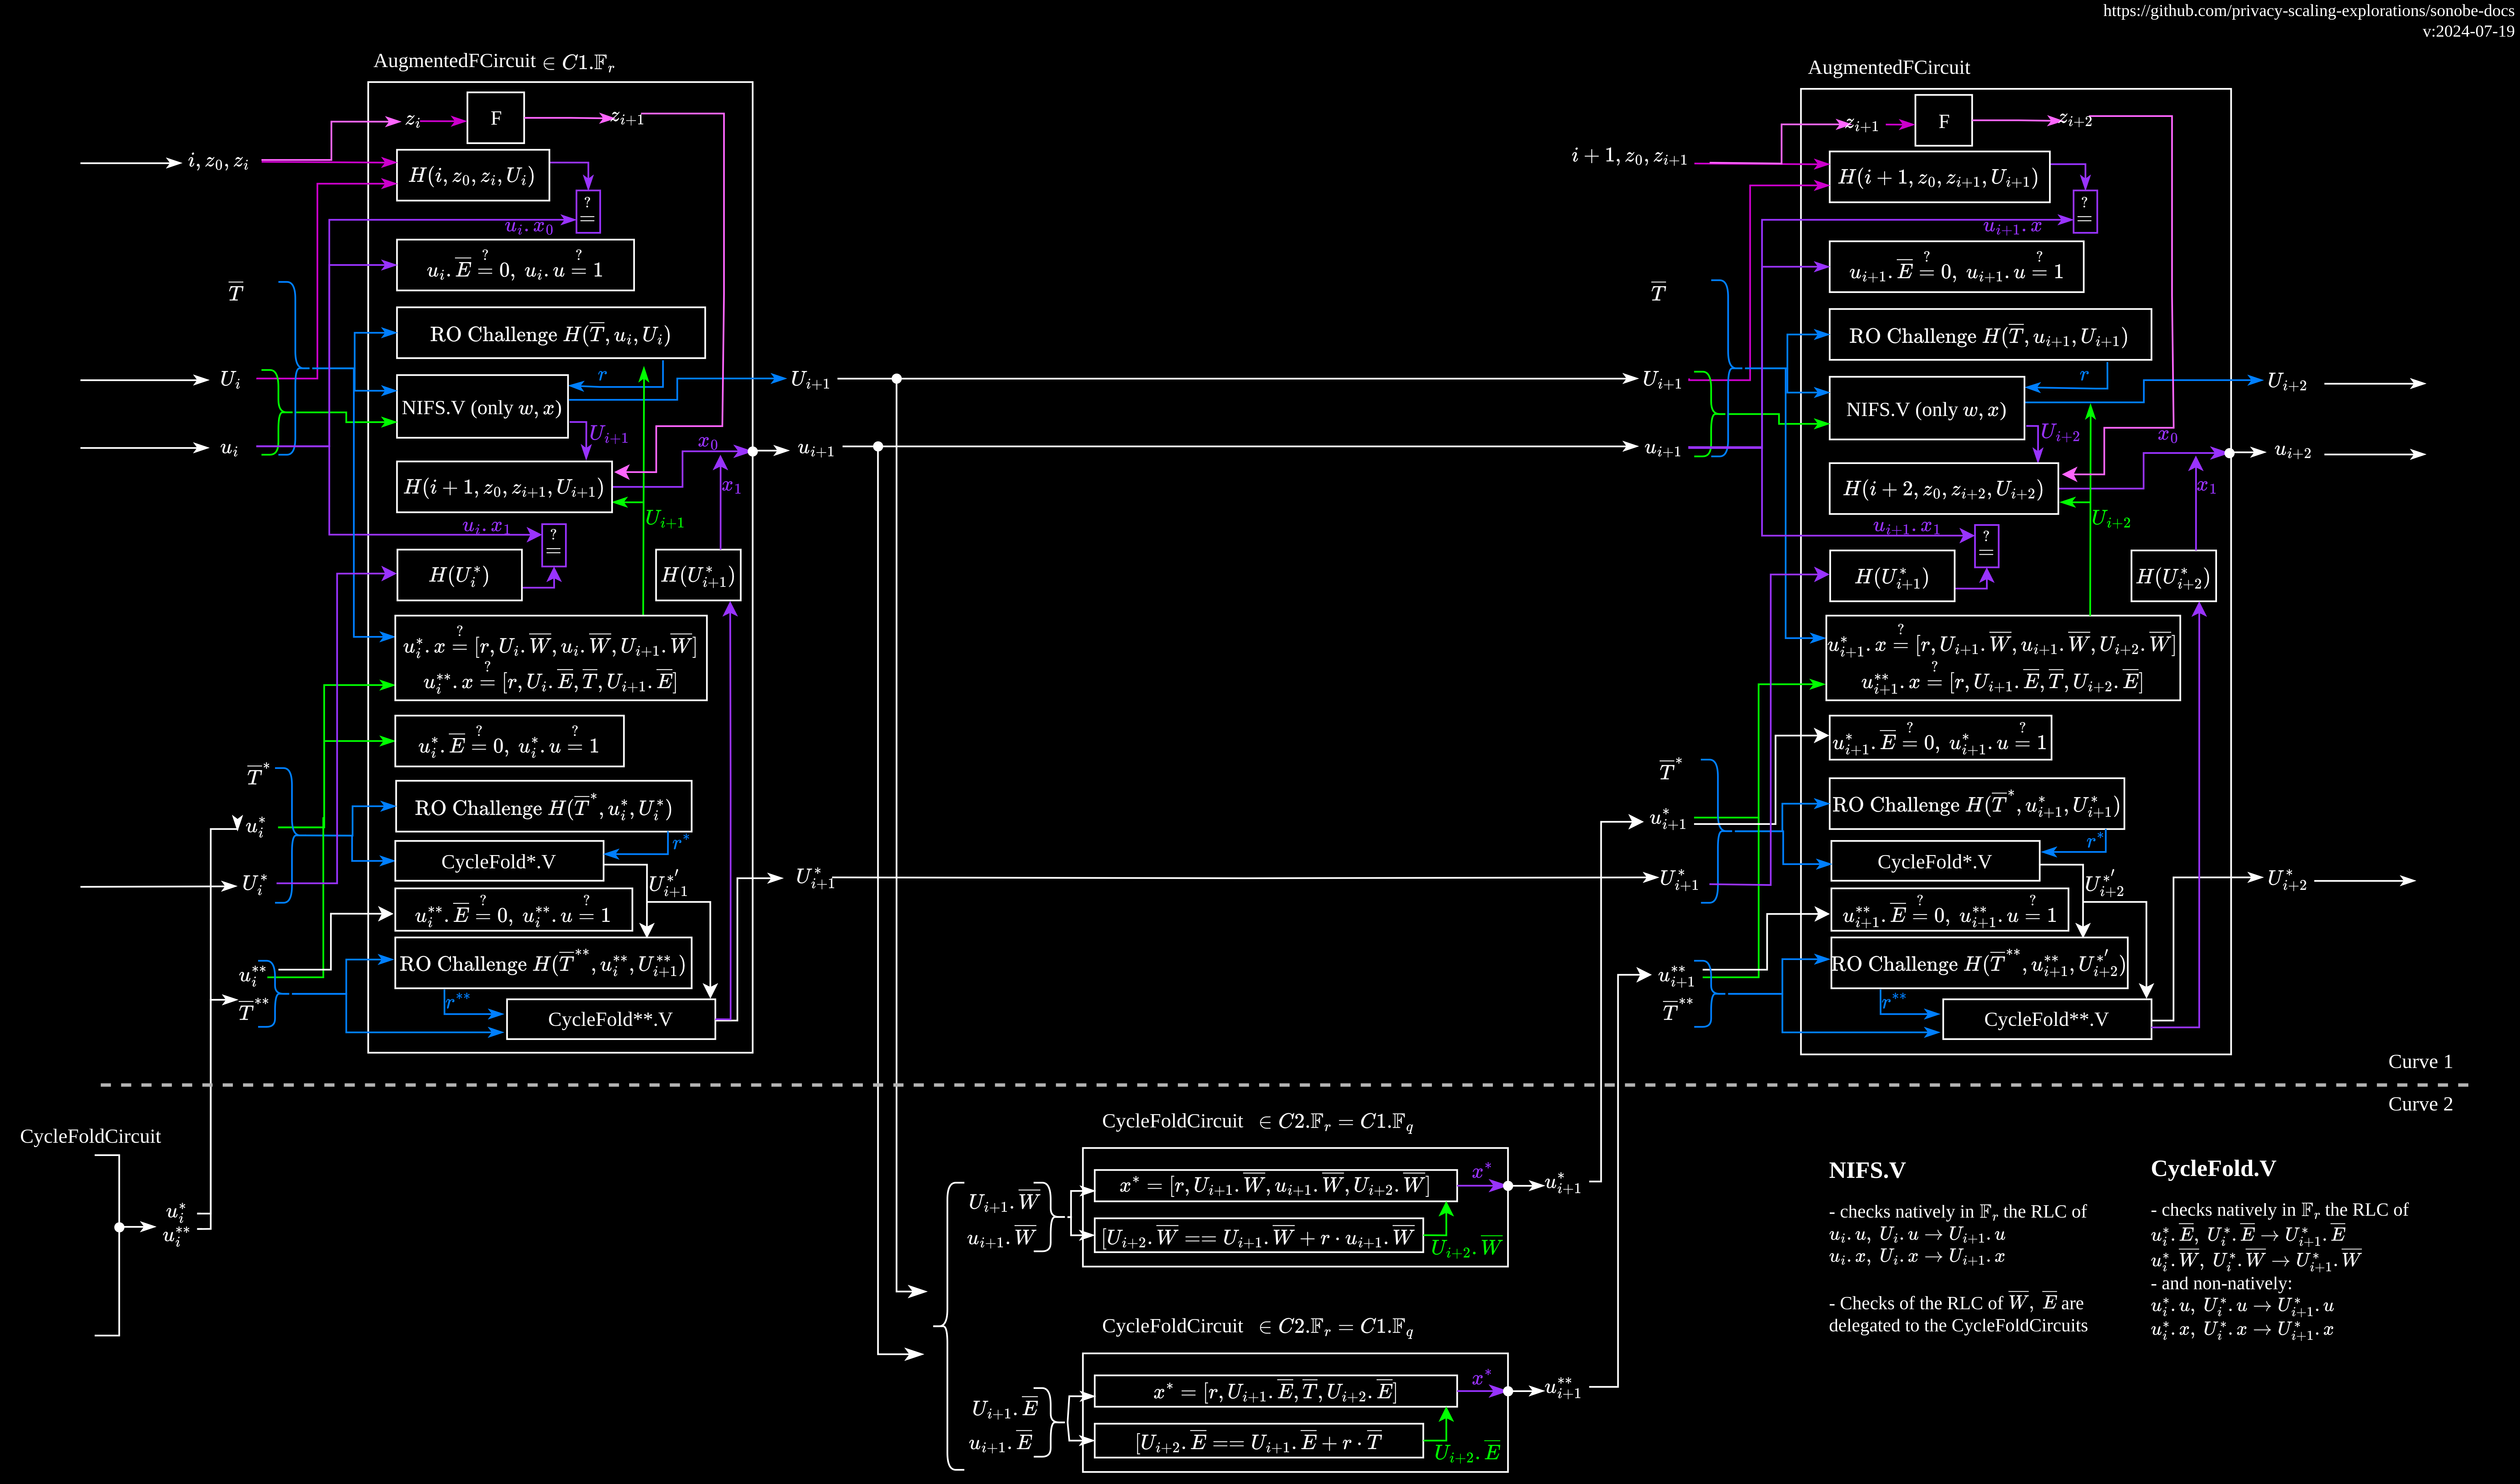
\includegraphics[width=\paperwidth]{cyclefold-nova-diagram}}
\begin{frame}[plain]
  \vskip0pt plus 1filll
  {\tiny 
    Nova's Folding Circuit (F') + CycleFold circuit

    src: \href{https://privacy-scaling-explorations.github.io/sonobe-docs/design/novacyclefold-circuit.html}{https://privacy-scaling-explorations.github.io/sonobe-docs/design/novacyclefold-circuit.html}
  }
\end{frame}
}
% \begin{frame}{Augmented F Circuit + CycleFold Circuit}
% \begin{frame}
% \begin{tikzpicture}
%   \node at (current page.center) {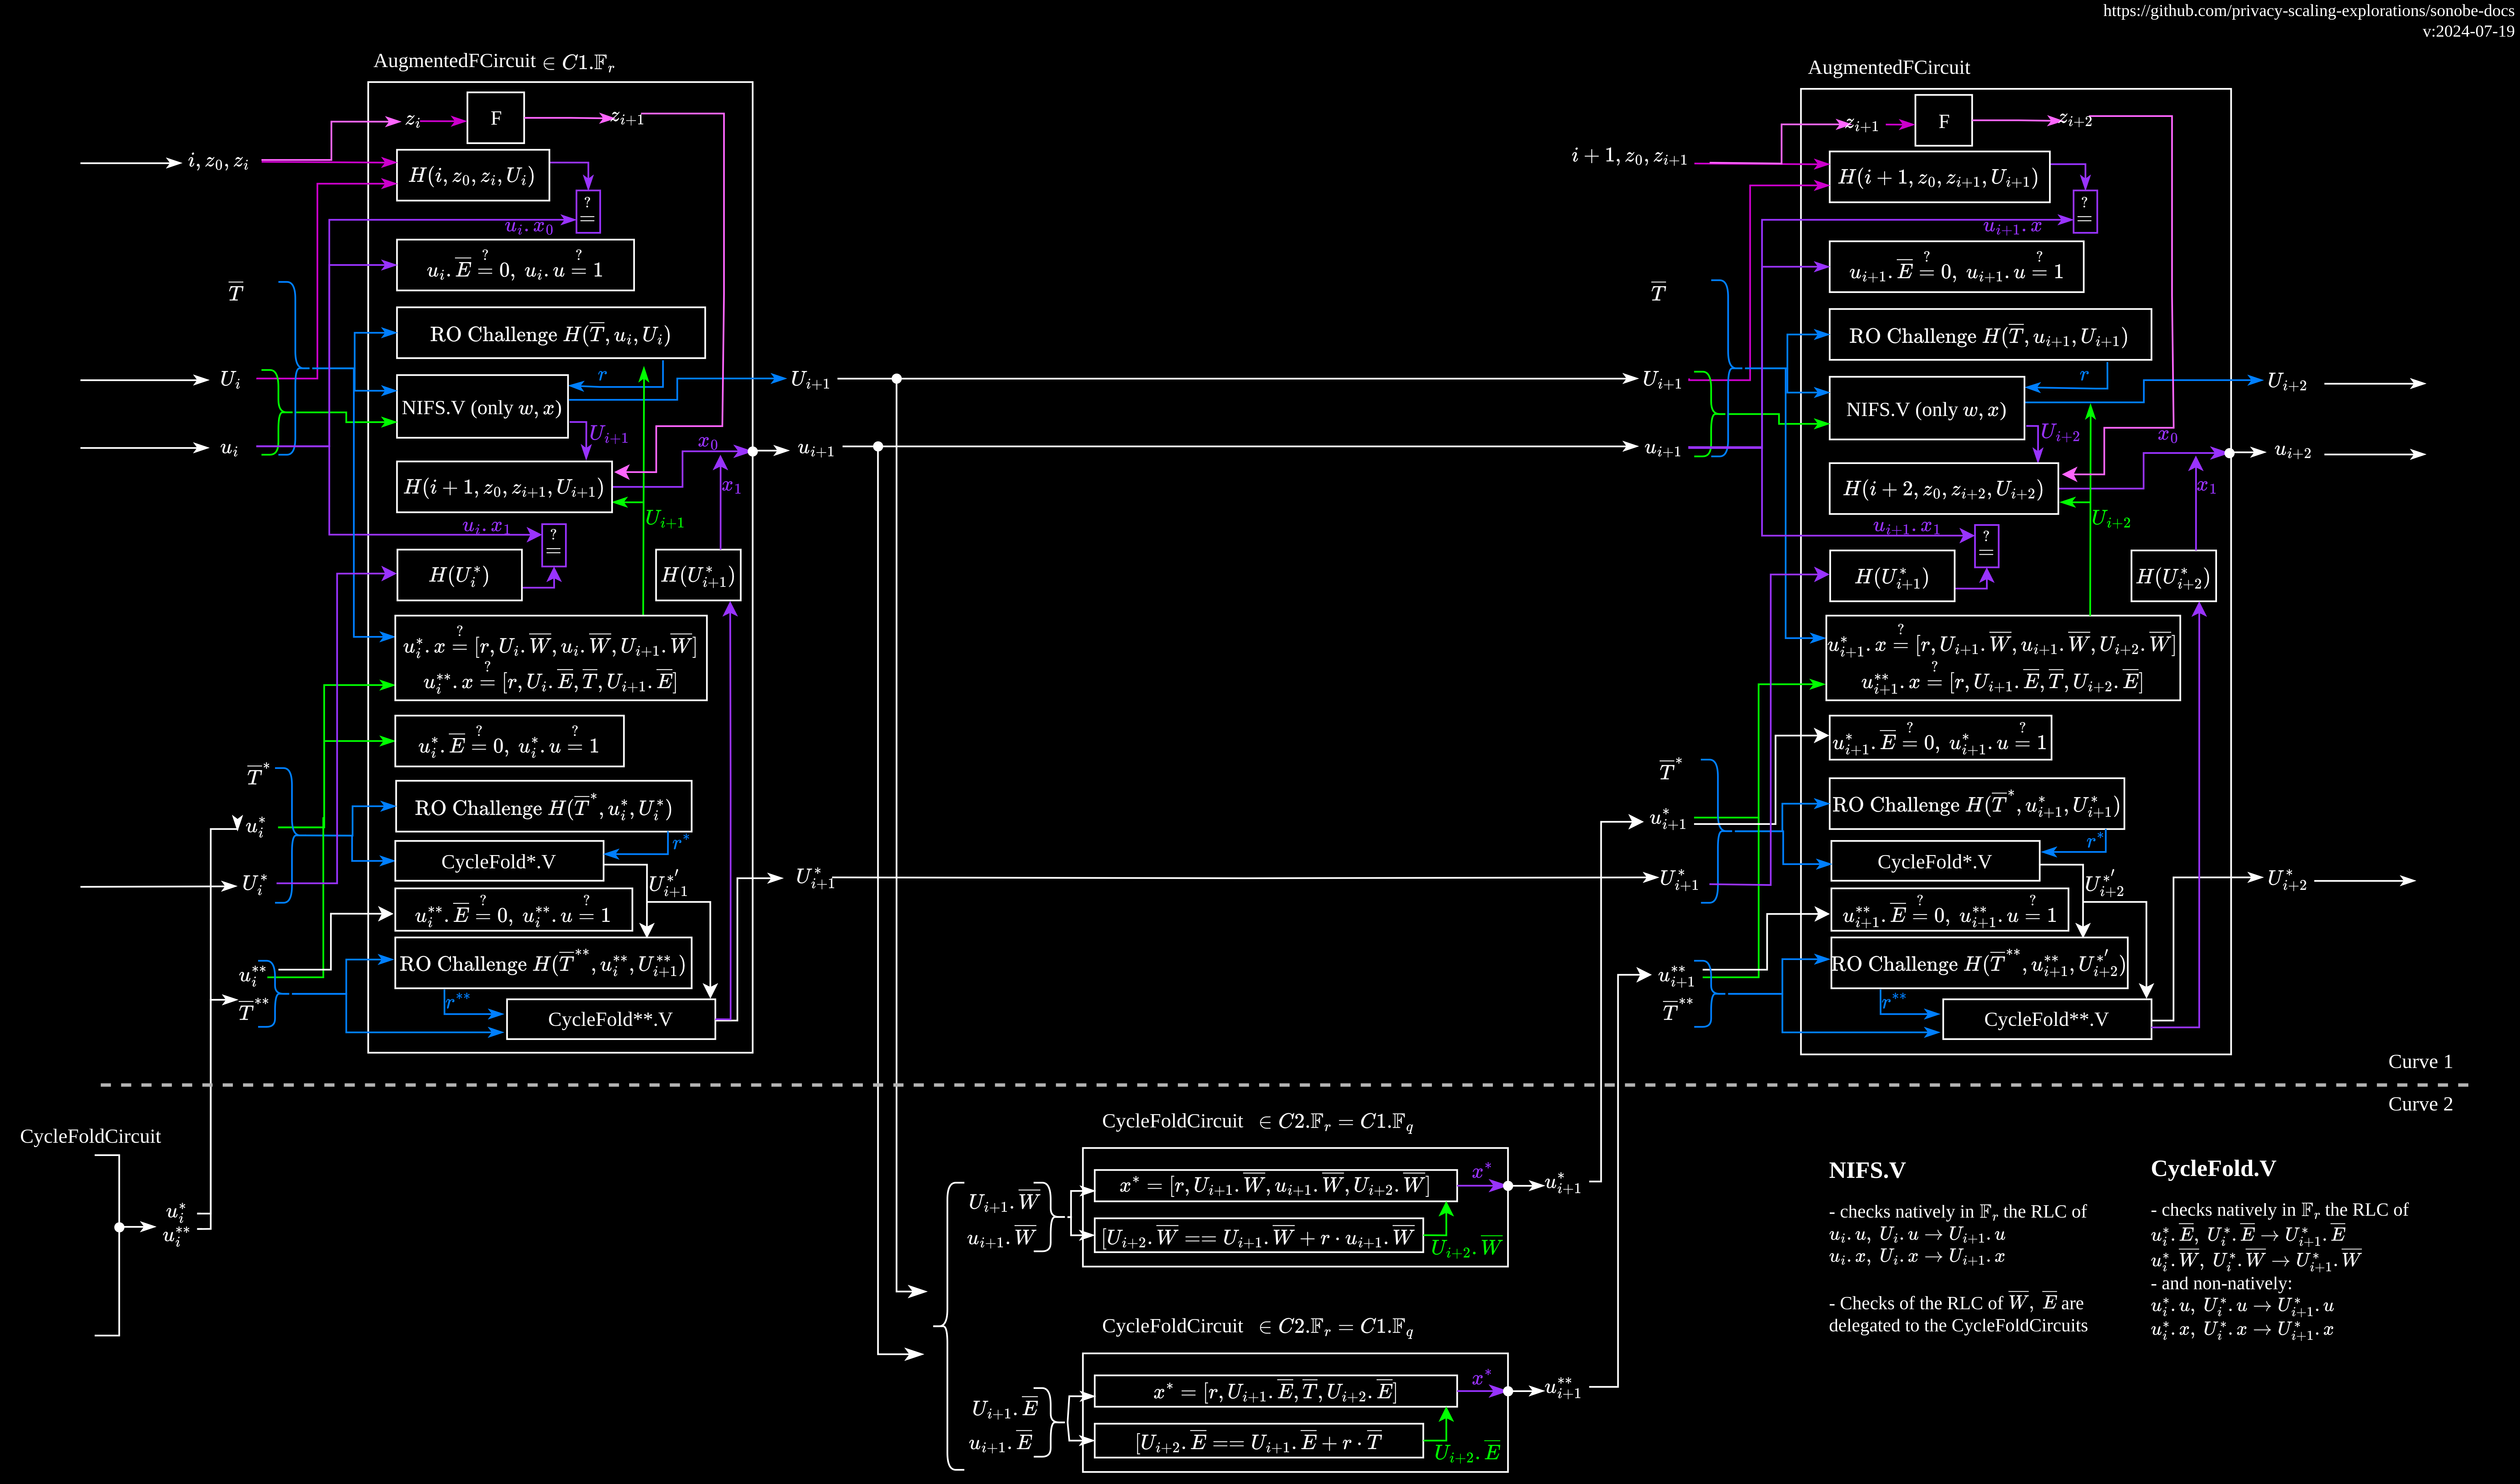
\includegraphics[width=\paperwidth, height=\paperheight]{cyclefold-nova-diagram}}
% \end{tikzpicture}
%   % 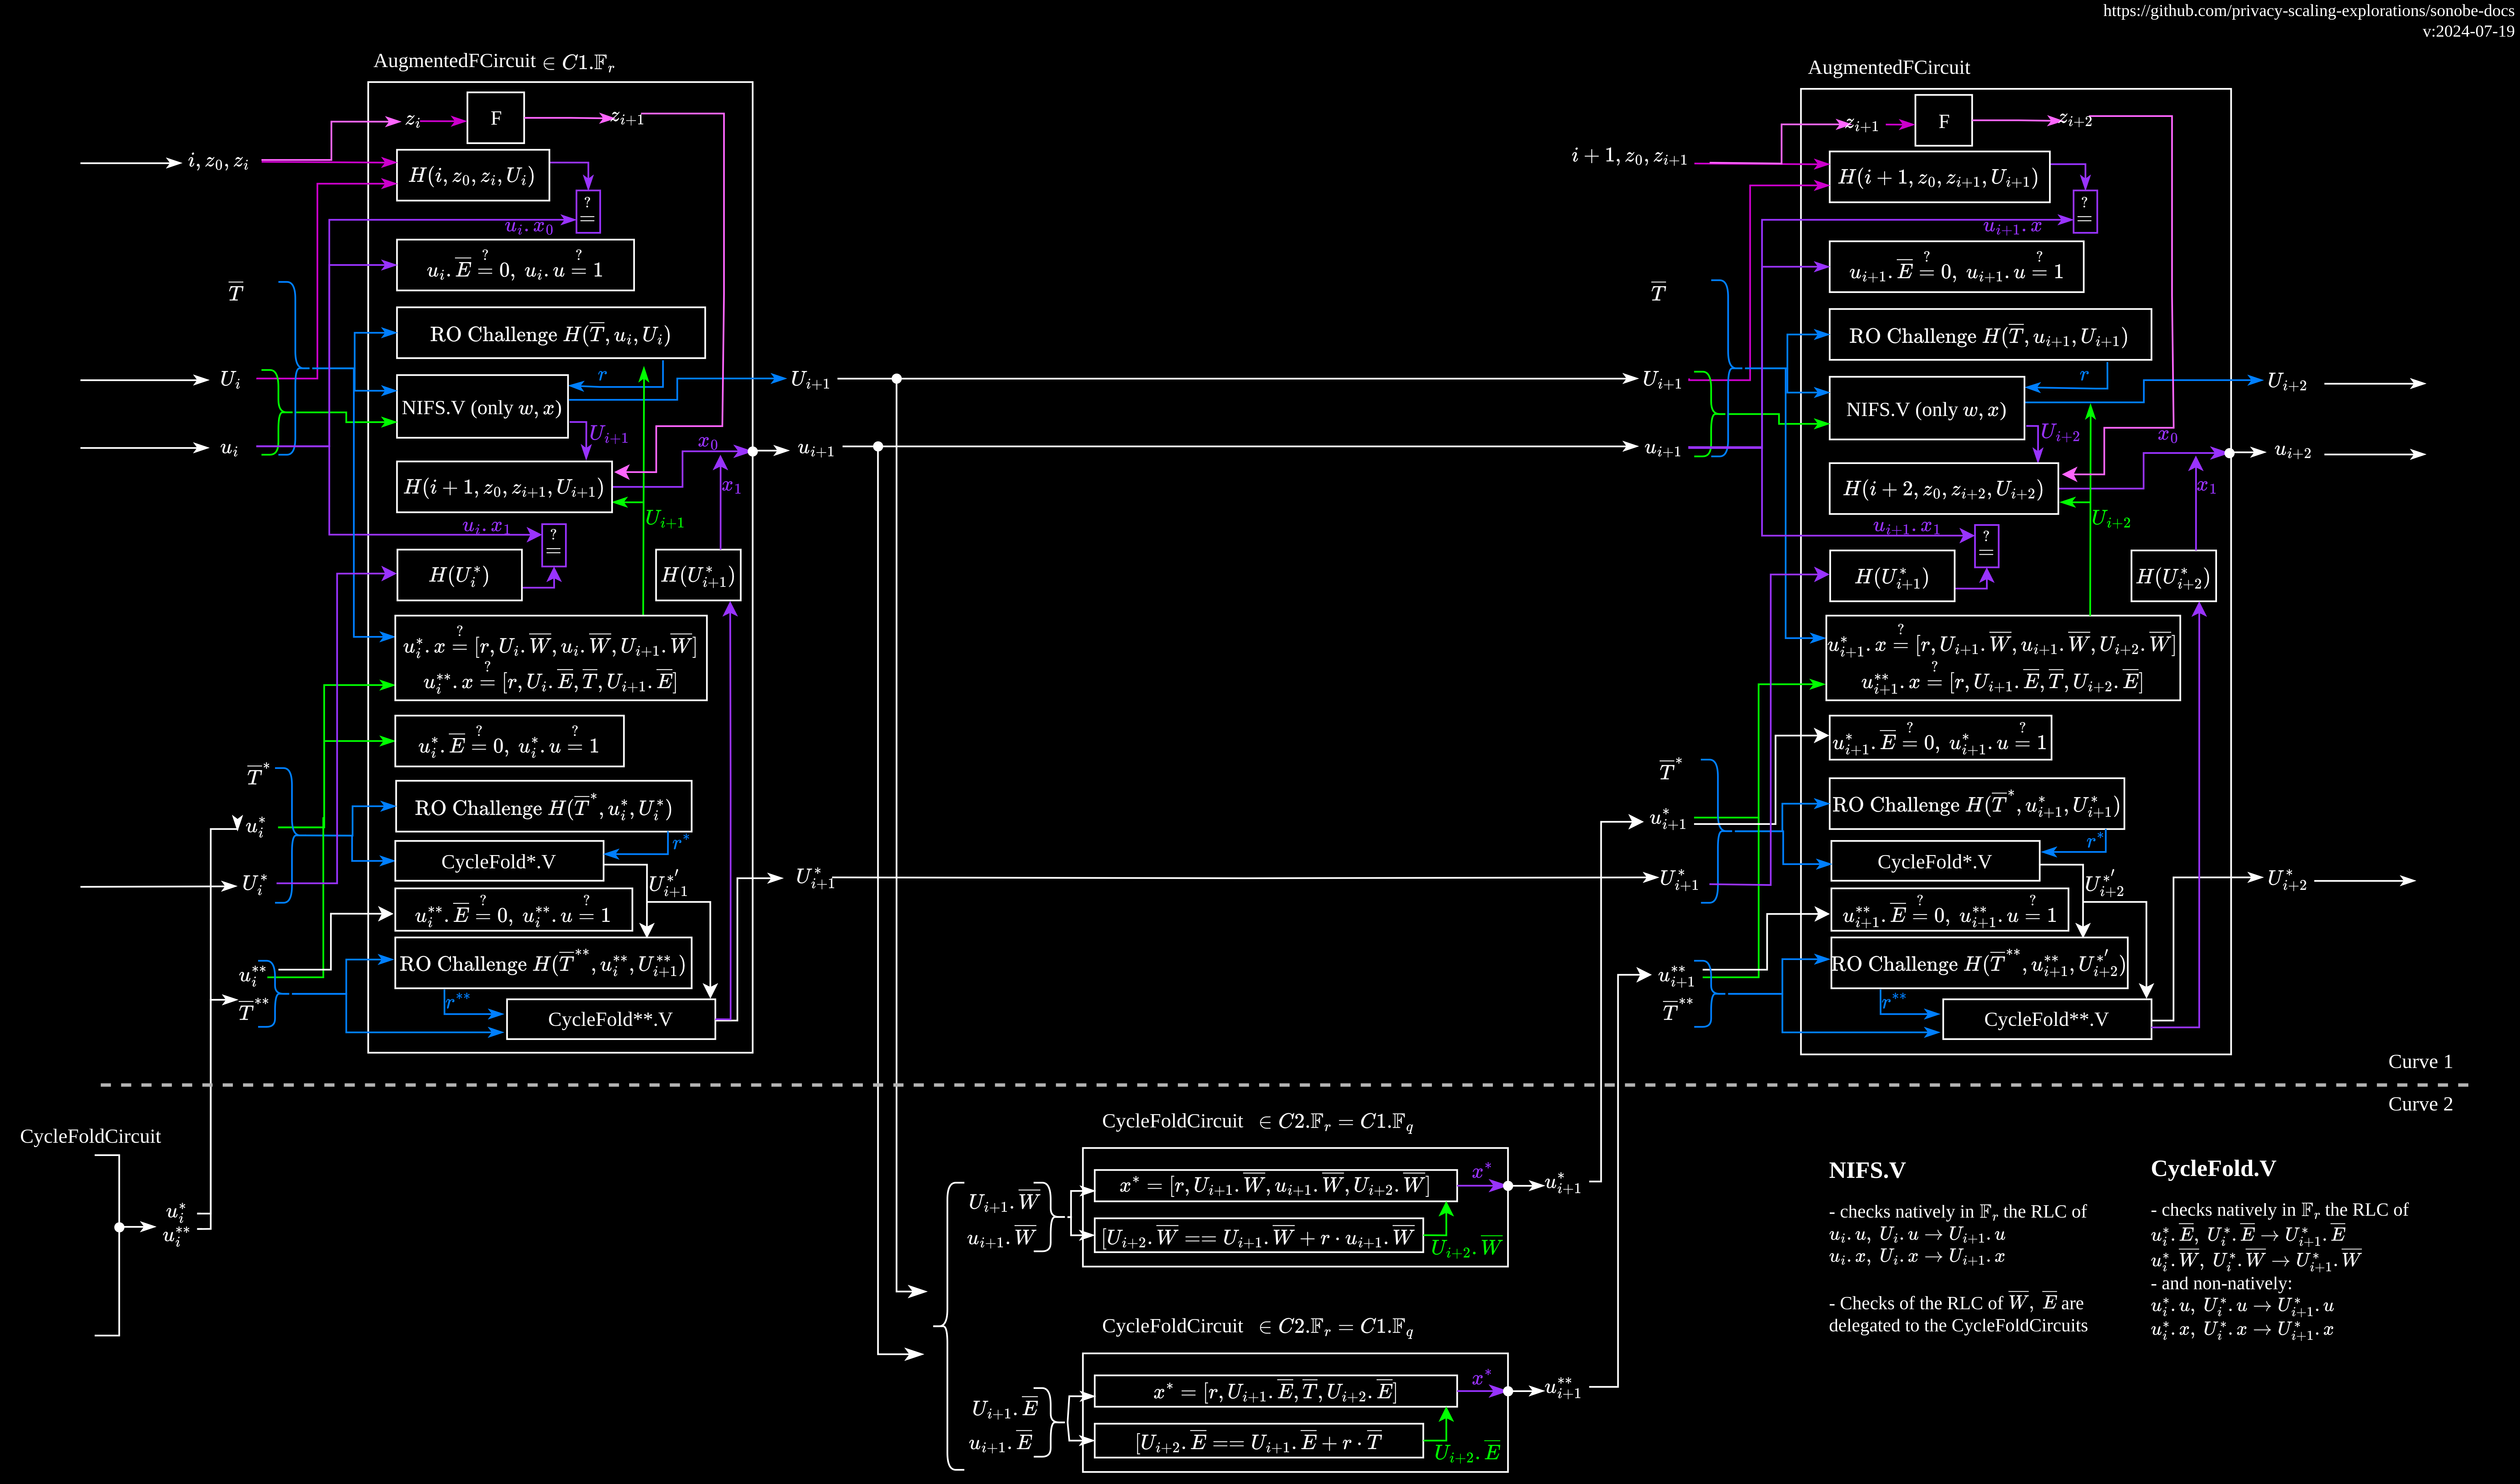
\includegraphics[width=\textwidth]{cyclefold-nova-diagram}
%   % {\tiny src: \href{https://privacy-scaling-explorations.github.io/sonobe-docs/design/novacyclefold-circuit.html}{https://privacy-scaling-explorations.github.io/sonobe-docs/design/novacyclefold-circuit.html}}
%   % mention TODO folding overhead - num constraints of overhead, so for small circuits it is not worth
%   % TODO explain: circuit overhead.
% \end{frame}


\section{Decider}

\begin{frame}{(Recall) Folding scheme pipeline}
  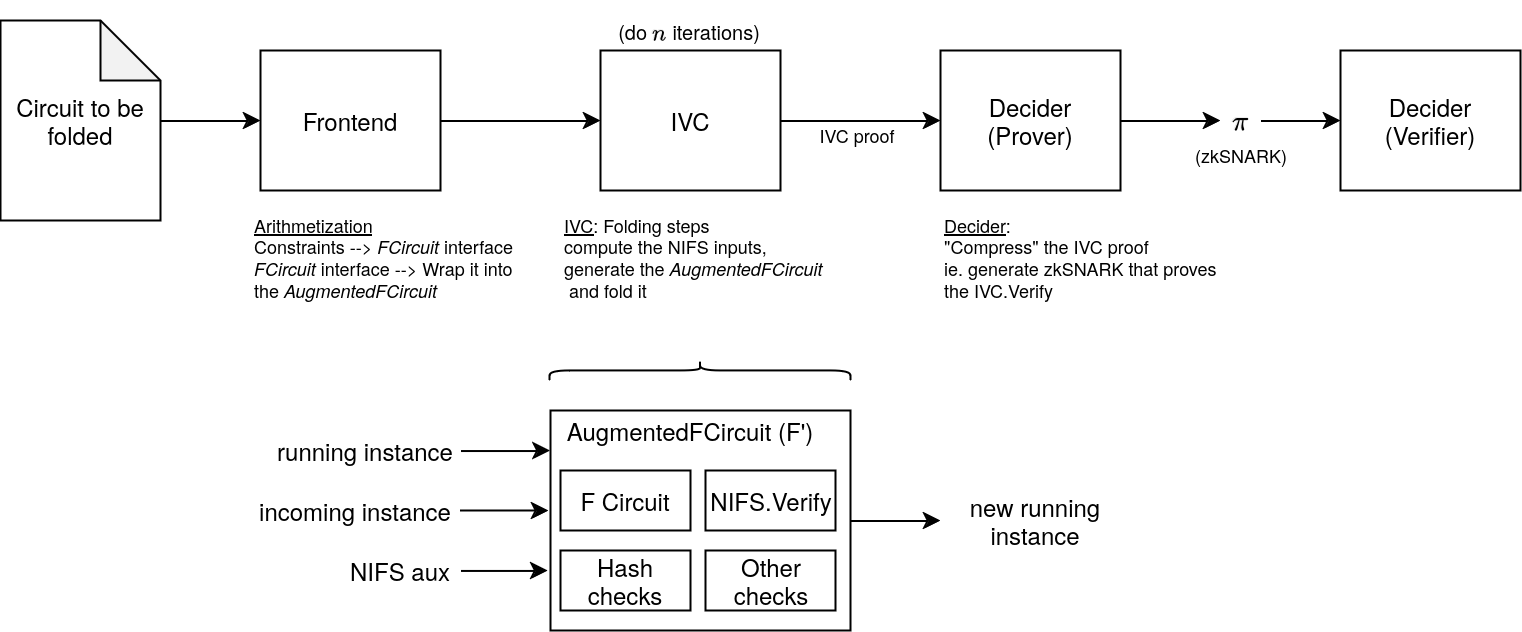
\includegraphics[width=\textwidth]{folding-scheme-pipeline}

  \vspace{0.5cm}
  {\scriptsize
  The IVC folds the AugmentedFCircuit, which ensures that the NIFS.Verify checks out.
  }
\end{frame}


\begin{frame}{Decider (Final compressed proof)}
  \vspace{-0.5cm}
  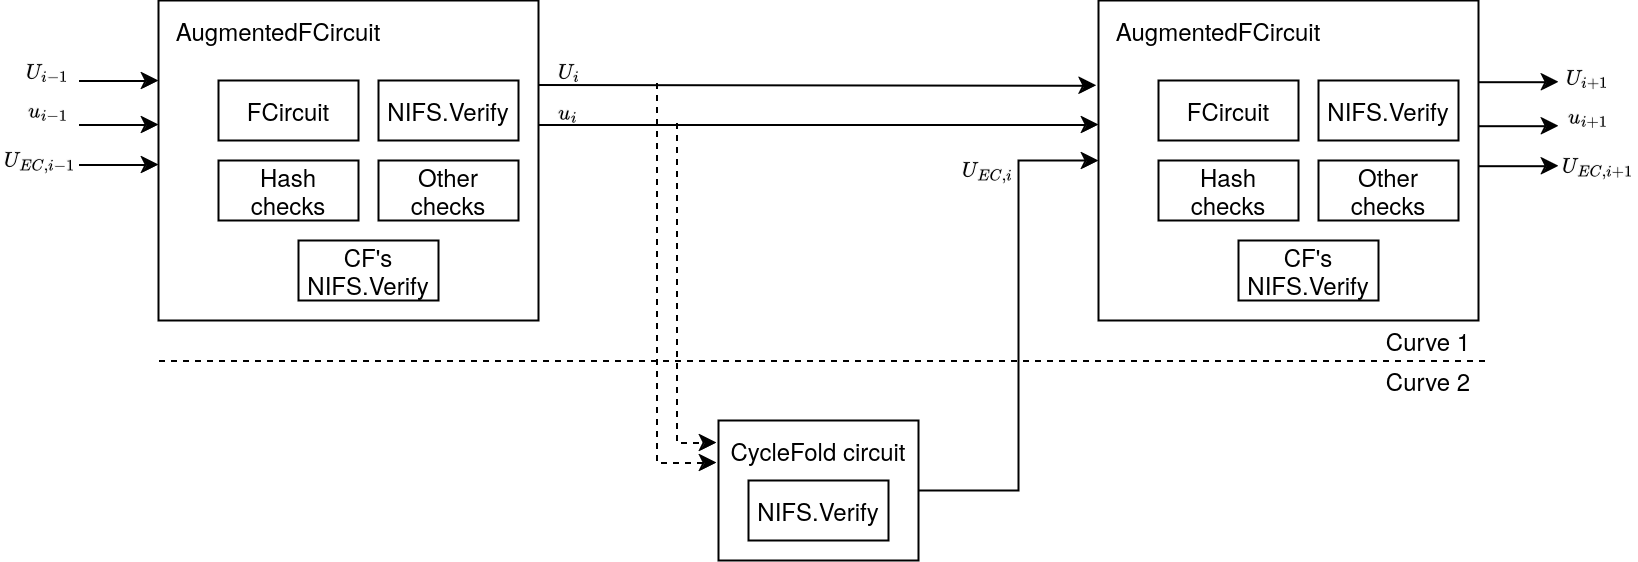
\includegraphics[width=\textwidth]{decider-instances}

  {\scriptsize
  Issue: IVC proof is not succinct.
  \begin{itemize}
    \item Committed Instances of the AugmentedFCircuit $U_n$, $u_n$, where each one is $\{ \overline{E} \in \mathbb{G}_1, \overline{W} \in \mathbb{G}_1, u \in \mathbb{F}_r, x \in \mathbb{F}_r^{|io|} \}$
    \item and their respective Witnesses $W_n, w_n$, each one being $\{E \in \mathbb{F}_r^n, W \in \mathbb{F}_r^n \}$
    \item Committed instance of the CycleFold circuit $U_{EC,n}$ contains: $\{ \overline{E} \in \mathbb{G}_2, \overline{W} \in \mathbb{G}_2, u \in \mathbb{F}_q, x \in \mathbb{F}_q^{|io|} \}$
    \item and its Witnesses $W_{EC,n}$, being $\{E \in \mathbb{F}_r^n, W \in \mathbb{F}_r^n \}$
  \end{itemize}
  So the idea is to 'compress' the IVC proof into a zkSNARK proof, minimizing the size and the verifier computation.
  }

\end{frame}

% TODO rm
% \begin{frame}{Decider}
%   Original Nova: generate a zkSNARK proof with Spartan for $U_n, u_n, U_{EC, n}$\\
%   $\longrightarrow$ 2 Spartan proofs, one on each curve\\
%   (not EVM-friendly)
% 
%   \vspace{0.5cm}
% 
%   We need to do a bit of gymnastics to verify the folding proofs in Ethereum
% 
%   % TODO
%   % DRAW of the 2 circuits over the curves, and how we generate a Spartan proof for each one
% \end{frame}

\begin{frame}{Decider checks}
  \begin{enumerate}
    \item[1.] check $NIFS.V(r, U_n, u_n, \overline{T}) \stackrel{?}{=} U_{n+1}$
    \item[2.] check that $u_n.\overline{E}=0$ and $u_n.u=1$
    \item[3.] check that $u_n.x_0 = H(n, z_0, z_n, U_n)$ and $u_n.x_1 = H(U_{EC,n})$
    \item[4.] correct RelaxedR1CS relation of $U_{n+1}, W_{n+1}$ of the AugmentedFCircuit
    \item[5.] check commitments of $U_{n+1}.\{ \overline{E}, \overline{W} \}$ with respect $W_{n+1}$ (where $\overline{E}, \overline{W} \in E_1$)
    \item[6.] check the correct RelaxedR1CS relation of $U_{EC,n}, W_{EC,n}$ of the CycleFoldCircuit
    \item[7.] check commitments of $U_{EC,n}.\{ \overline{E}, \overline{W} \}$ with respect $W_{EC,n}$ (where $\overline{E},\overline{W} \in E_2$)
  \end{enumerate}
\end{frame}

\begin{frame}{Decider checks}
  \begin{enumerate}
    \item[1.] check $NIFS.V(r, U_n, u_n, \overline{T}) \stackrel{?}{=} U_{n+1}$
    \item[2.] check that $u_n.\overline{E}=0$ and $u_n.u=1$
    \item[3.] check that $u_n.x_0 = H(n, z_0, z_n, U_n)$ and $u_n.x_1 = H(U_{EC,n})$
    \item[4.] correct RelaxedR1CS relation of $U_{n+1}, W_{n+1}$ of the AugmentedFCircuit
    \item[5.] check commitments of $U_{n+1}.\{ \overline{E}, \overline{W} \}$ with respect $W_{n+1}$ (where $\overline{E}, \overline{W} \in E_1$) \textcolor{cyan}{non-native!}
    \item[6.] check the correct RelaxedR1CS relation of $U_{EC,n}, W_{EC,n}$ of the CycleFoldCircuit \textcolor{cyan}{non-native!}
    \item[7.] check commitments of $U_{EC,n}.\{ \overline{E}, \overline{W} \}$ with respect $W_{EC,n}$ (where $\overline{E},\overline{W} \in E_2$)
  \end{enumerate}
\end{frame}

\begin{frame}{Original Nova Decider}
  \begin{itemize}
    \item Original Nova: wrapp these checks in 2 Spartan (zkSNARK) proofs (one over each curve of the cycle of curves).\\
      $\longrightarrow$ 2 Spartan proofs, one on each curve\\
    \item In our case we were interested into verifying the proofs in Ethereum's EVM.
  \end{itemize}

  Need to do a bit of gymnastics to verify the folding proofs in Ethereum,\\
  EVM limitations:
  \begin{itemize}
    \item limited to BN254 curve
    \item constrainted by gas costs
  \end{itemize}
\end{frame}

\begin{frame}{Onchain Decider}
{\tiny
  \begin{enumerate}
    \item[1.1:] check that the given NIFS challenge $r$ is indeed well computed.
      \\This challenge is then used outside the circuit by the Verifier to compute NIFS.V obtaining $U_{i+1}$
    \item[2:] check that $u_n.\overline{E}=0$ and $u_n.u=1$
    \item[3:] check that $u_n.x_0 = H(n, z_0, z_n, U_n)$ and $u_n.x_1 = H(U_{EC,n})$
    \item[4:] correct RelaxedR1CS relation of $U_{n+1}, W_{n+1}$ of the AugmentedFCircuit
    \item[5.1:] Check correct computation of the KZG challenges
      \\$c_E = H(\overline{E}.\{x,y\}),~~c_W = H(\overline{W}.\{x,y\})$
      \\which we do through in-circuit Transcript.
    \item[5.2:] check that the KZG evaluations are correct, $eval_W == p_W(c_W),~~ eval_E == p_E(c_E)$
      \\where $p_W, p_E \in \mathbb{F}[X]$ are the interpolated polynomials from $W_{i+1}.W,~ W_{i+1}.E$ respectively.
    \item[6:] check the correct RelaxedR1CS relation of $U_{EC,n}, W_{EC,n}$ of the CycleFoldCircuit
      \\(this is non-native operations and with naive sparse matrix-vector product blows up the number of constraints)
    \item[7:] Pedersen commitments verification of $U_{EC,n}.\{ \overline{E}, \overline{W} \}$ with respect $W_{EC,n}$
      \\(the witness of the committed instance)
  \\(where $\overline{E},\overline{W} \in E_2$, this check is native in $F_r$)
  \end{enumerate}

  \emph{The following check is done non-natively (in $F_r$):}
  Additionally we would have to check (outside of the circuit):

  \begin{enumerate}
    \item[1.2:] check $NIFS.V(r, U_n, u_n, \overline{T}) \stackrel{?}{=} U_{n+1}$
    \item[5.3:] Commitments verification of $U_{n+1}.\{ \overline{E}, \overline{W} \}$ with respect $W_{n+1}$ (where $\overline{E}, \overline{W} \in E_1$)
  \end{enumerate}

  {\tiny More details in Sonobe's docs: \href{https://privacy-scaling-explorations.github.io/sonobe-docs/design/novacyclefold-circuit.html}{https://privacy-scaling-explorations.github.io/sonobe-docs/design/novacyclefold-circuit.html}}
}
\end{frame}

\begin{frame}{Onchain Decider}
  % DRAW of the full flow: from inputting the circuit, to folding to generating the Decider proof to verifying in Ethereum
  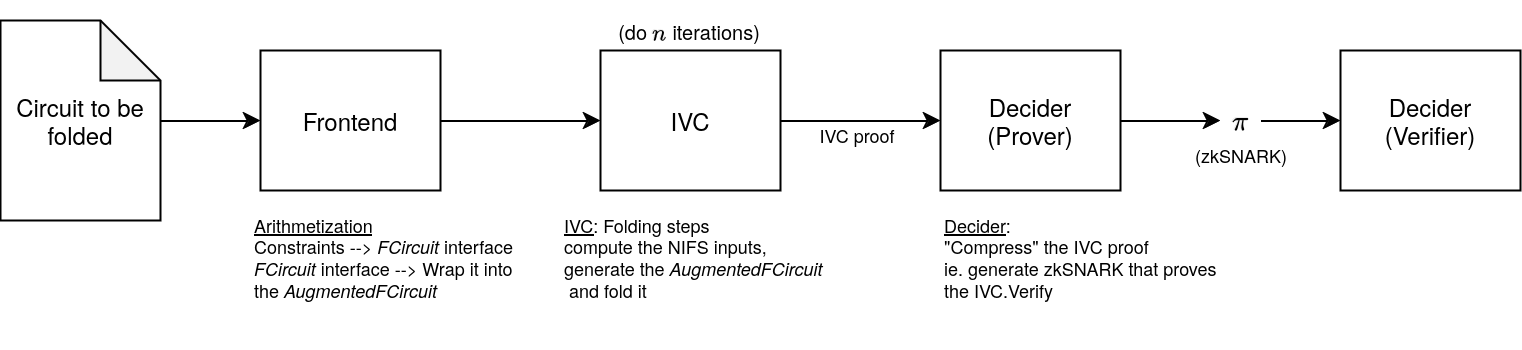
\includegraphics[width=8cm]{folding-scheme-pipeline-without-augmentedfcircuit}
  \pause
  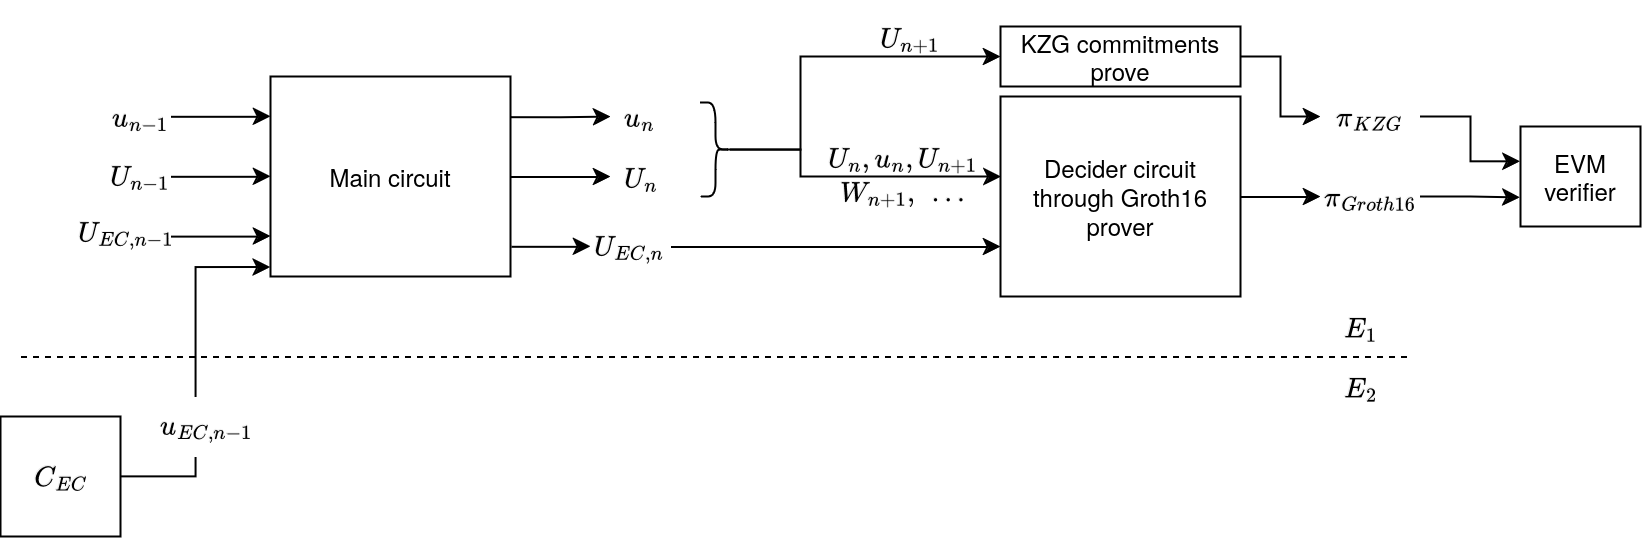
\includegraphics[width=\textwidth]{decider-onchain-flow-diagram}
\end{frame}


% TODO maybe remove
% \begin{frame}{Offchain Decider}
%   {\tiny
%     \textbf{Circuit1} $\in \mathbb{F}_r$ ($E_1.\mathbb{F}_r$):
%   \begin{enumerate}
%     \item[1.1:] check that the given NIFS challenge $r$ is indeed well computed.
%       \\This challenge is then used outside the circuit by the Verifier to compute NIFS.V obtaining $U_{i+1}$
%     \item[2:] check that $u_n.\overline{E}=0$ and $u_n.u=1$
%     \item[3:] check that $u_n.x_0 = H(n, z_0, z_n, U_n)$ and $u_n.x_1 = H(U_{EC,n})$
%     \item[4:] correct RelaxedR1CS relation of $U_{n+1}, W_{n+1}$ of the AugmentedFCircuit
%     \item[5.1:] Check correct computation of the CommitmentScheme challenges for $U_{n+1}$
%       \\$$c_E = H(U_{n+1}.\overline{E}.\{x,y\}),~~c_W = H(U_{n+1}.\overline{W}.\{x,y\})$$
%       \\which we do through in-circuit Transcript.
%     \item[5.2:] check that the CommitmentScheme evaluations for $U_{n+1}$ are correct, $eval_W == p_W(c_W),~~~ eval_E == p_E(c_E)$
%       \\where $p_W, p_E \in \mathbb{F}[X]$ are the interpolated polynomials from $W_{i+1}.W,~ W_{i+1}.E$ respectively.
%   \end{enumerate}
% 
%   \textbf{Circuit2} $\in \mathbb{F}_q$ ($E_2.\mathbb{F}_r$):
%   \begin{enumerate}
%     \item[6:] correct RelaxedR1CS relation of $U_{EC,d}, W_{EC,d}$
%     \item[7.1:] Check correct computation of the CommitmentScheme challenges for $U_{EC}$
%       \\$$c_E = H(U_{EC}.\overline{E}.\{x,y\}),~~c_W = H(U_{EC}.\overline{W}.\{x,y\})$$
%       \\which we do through in-circuit Transcript.
%     \item[7.2:] check that the CommitmentScheme evaluations for $U_{EC}$ are correct
%       - $eval_W == p_W(c_W)$
%       - $eval_E == p_E(c_E)$
%       \\where $p_W, p_E \in \mathbb{F}[X]$ are the interpolated polynomials from $W_{i+1}.W,~ W_{i+1}.E$ respectively.
%   \end{enumerate}
% 
%   \textbf{Outside the circuits}:
%   \begin{enumerate}
%     \item[1.2:] check $NIFS.V(r, U_d, u_d, \overline{T}) \stackrel{?}{=} U_{d+1}$
%     \item[5.3:] Commitments verification of $U_{d+1}.\{ \overline{E}, \overline{W} \}$
%       \\with respect $W_{d+1}$ (where $\overline{E}, \overline{W} \in E_1$)
%     \item[7.3:] Commitments verification of $U_{EC,d}.\{ \overline{E}, \overline{W} \}$
%       \\with respect $W_{EC,d}$ 
%     \\(where $\overline{E},\overline{W} \in E_2$)
%   \end{enumerate}
% }
% TODO fix that currently it does not fit in the slide

\end{frame}


\section{Sonobe}

\begin{frame}{Sonobe}

  \footnotesize{
  Experimental folding schemes library implemented jointly by 0xPARC and PSE.\\
  \href{https://github.com/privacy-scaling-explorations/sonobe}{https://github.com/privacy-scaling-explorations/sonobe}
  \\Modular library,
  \begin{itemize}
    \item Be able to
    \begin{itemize}
      \item Add and test new folding schemes
      \item Compare schemes 'apples-to-apples'
      \item Researchers can easily add their own schemes (eg. Mova paper)
    \end{itemize}
    \item Make it easy for devs to use folding
    \begin{itemize}
      \item minimal code to fold your circuits ('plug-and-fold')
      \item easy to switch between folding schemes and curves
      \item support of multiple zk-circuit languages
    \end{itemize}
  \end{itemize}

  \vspace{0.5cm}
  \emph{Remark}: experimental and unoptimized.
  }
\end{frame}

\begin{frame}{Sonobe - Dev experience}
  \scriptsize{

  Dev flow:
  \begin{enumerate}
    \item Define a circuit to be folded
    \item Set which folding scheme to be used (eg. Nova with CycleFold)
    \item Set a final decider to generate the final proof (eg. Groth16 over BN254 curve)
    \item Generate the Solidity decider verifier (EVM Solidity contract)
  \end{enumerate}
  }

  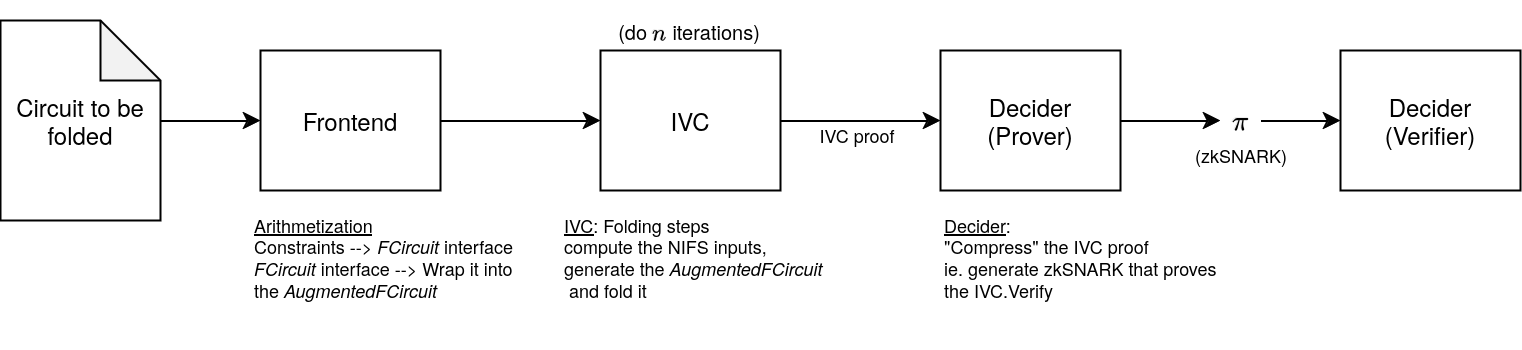
\includegraphics[width=\textwidth]{folding-scheme-pipeline-without-augmentedfcircuit}
  Sonobe lib pipeline:
  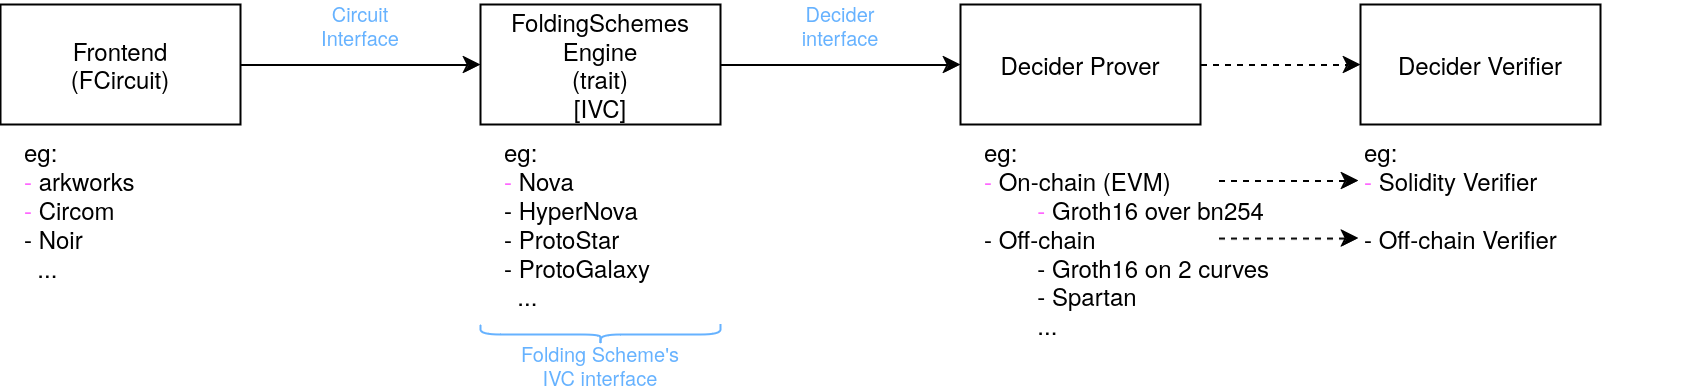
\includegraphics[width=\textwidth]{sonobe-lib-pipeline}
\end{frame}


\begin{frame}{Status of Sonobe - schemes implemented}
  \scriptsize{
  Implemented (fully implemented):
  \begin{itemize}
    \item \textbf{Nova}: Recursive Zero-Knowledge Arguments from Folding Schemes\\ \href{https://eprint.iacr.org/2021/370.pdf}{https://eprint.iacr.org/2021/370.pdf}, Abhiram Kothapalli, Srinath Setty, Ioanna Tzialla. 2021
    \item \textbf{CycleFold}: Folding-scheme-based recursive arguments over a cycle of elliptic curves\\ \href{https://eprint.iacr.org/2023/1192.pdf}{https://eprint.iacr.org/2023/1192.pdf}, Abhiram Kothapalli, Srinath Setty. 2023
    \item \textbf{HyperNova}: Recursive arguments for customizable constraint systems\\ \href{https://eprint.iacr.org/2023/573.pdf}{https://eprint.iacr.org/2023/573.pdf}, Abhiram Kothapalli, Srinath Setty. 2023
    \item \textbf{ProtoGalaxy}: Efficient ProtoStar-style folding of multiple instances\\ \href{https://eprint.iacr.org/2023/1106.pdf}{https://eprint.iacr.org/2023/1106.pdf}, Liam Eagen, Ariel Gabizon. 2023
  \end{itemize}
  {\tiny
    Started (NIFS implemented, next: folding circuit, IVC, Decider, etc):
    \begin{itemize}
     \item \textbf{Mova}: Nova folding without committing to error terms\\ \href{https://eprint.iacr.org/2024/1220.pdf}{https://eprint.iacr.org/2024/1220.pdf}, Nikolaos Dimitriou, Albert Garreta, Ignacio Manzur, Ilia Vlasov. 2024
     \item \textbf{Ova}: Reduce the accumulation verifier in Nova from 2 to just 1 group operation\\ \href{https://eprint.iacr.org/2024/1220.pdf}{https://eprint.iacr.org/2024/1220.pdf}, Benedikt Bünz. 2024
    \end{itemize}
  }

  Frontends - how can the dev define a circuit to be folded
  \begin{itemize}
    \item Arkworks \href{https://github.com/arkworks-rs}{https://github.com/arkworks-rs}
    \item experimental: Circom, Noir, Noname.
  % Frontends - how can the dev define a circuit to be folded
  % \begin{itemize}
  %   \item Arkworks \href{https://github.com/arkworks-rs/}{https://github.com/arkworks-rs/}
  %   \item experimental:
  %   \begin{itemize}
  %     \item Circom \href{https://github.com/iden3/circom}{https://github.com/iden3/circom}
  %     \item Noir \href{https://noir-lang.org/}{https://noir-lang.org/}
  %     \item Noname \href{https://github.com/zksecurity/noname}{https://github.com/zksecurity/noname}
  %   \end{itemize}
  \end{itemize}

  }
\end{frame}

\begin{frame}{Modularity}
  % TODO
  Big thanks to arkworks \href{https://github.com/arkworks-rs}{https://github.com/arkworks-rs}

  \vspace{1cm}
  [Code example in the code editor]

\end{frame}

\begin{frame}{Some numbers}
  \footnotesize{
  (code highly unoptimized)
  \begin{itemize}
    \item folding step $\sim 300 ms$
      \begin{itemize}
      \item Folding circuit (Nova+CycleFold): $\sim 50k$ R1CS constraints (overhead)
      \end{itemize}
    \item Offchain Decider prove: $< 1$ min
    \item Onchain Decider Verification:
    \begin{itemize}
      \item DeciderEthCircuit: $\sim 10M$ R1CS constraints
      \begin{itemize}
        \item $<3$ minutes in a 32GB RAM 16 core laptop
      \end{itemize}
      \item gas costs (DeciderEthCircuit proof): $\sim 800k$ gas
      \begin{itemize}
        \item mostly from G16, KZG10, public inputs processing
        \item can be reduced by hashing the public inputs \& batching the pairings check
        \item expect to get it down to $< 500k$ gas.
      \end{itemize}
    \end{itemize}
  \end{itemize}
  }

  \vspace{0.6cm}

  Recall, this proof is proving that applying $n$ times the function $F$ (the circuit that we're folding) to an initial state $z_0$ results in the state $z_n$.
\end{frame}

\begin{frame}{Wrappup}
  \small{
  \begin{itemize}
    \item repo: \href{https://github.com/privacy-scaling-explorations/sonobe}{https://github.com/privacy-scaling-explorations/sonobe}
    \item docs: \href{https://privacy-scaling-explorations.github.io/sonobe-docs/}{https://privacy-scaling-explorations.github.io/sonobe-docs/}
  \end{itemize}
  }

  \begin{center}
    
\includegraphics[width=5cm]{./imgs/sonobe-link-qrcode}
  \end{center}

\tiny{
  $$\text{2024-10-08}$$
  $$\text{\href{https://0xparc.org}{0xPARC}~\&~\href{https://pse.dev/}{PSE.}}$$
}
\end{frame}

% \begin{frame}{NEWFRAME}
% \end{frame}
% 
% \begin{frame}{NEWFRAME}
% \end{frame}

\end{document}

% WORDS TO CHECK PRONOUNCIATION:
% - parallel
% - inherits
% - instances
% - sumcheck
% - R1CS
